\ifdefined\COMPLETE
\else
    \input{../preambule-utf8.ltx}   
\usepackage{tikz}                                   %
\usepackage{tkz-tab,tkz-euclide,tkz-fct,tkz-base}    % Pour les graphiques ch 2
\usetkzobj{all}
\usepackage[tikz]{bclogo}
    \begin{document}
\fi

%----------------------------------Page 1 ------------


\setbox1=\vbox{\hsize=9cm \begin{minipage}{9cm}
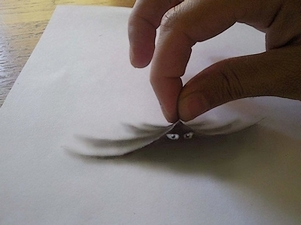
\includegraphics[width=9cm,height=90mm]{Soulever_la_question.jpg} 
\end{minipage}}
%----------------------------------Page 2 ------------


\setbox2=\vbox{\hsize=9cm \begin{minipage}{9cm}

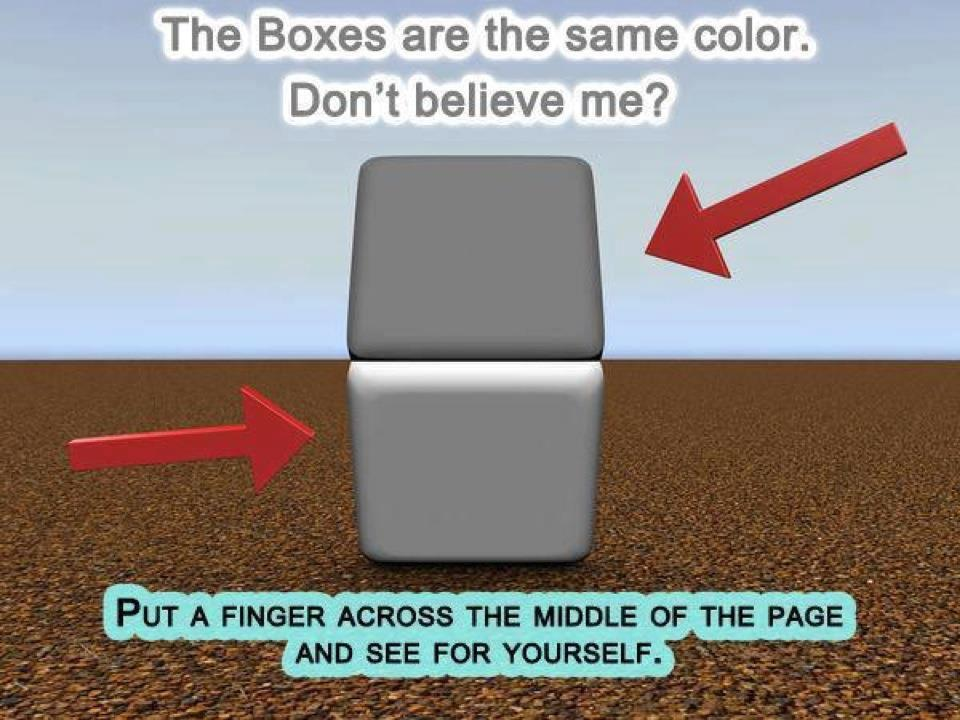
\includegraphics[width=9cm]{Same_color.jpg} 
\end{minipage}}
%----------------------------------Page 3 ------------

\setbox3=\vbox{\hsize=9cm \begin{minipage}{9cm}
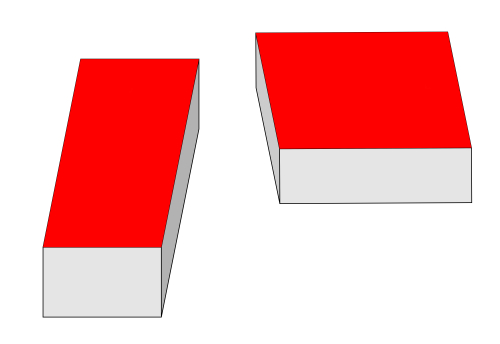
\includegraphics[width=9cm]{Shepardillusion.jpg} 
\end{minipage}}
%----------------------------------Page 4 ------------

\setbox4=\vbox{\hsize=9cm \begin{minipage}{9cm}
\centerline{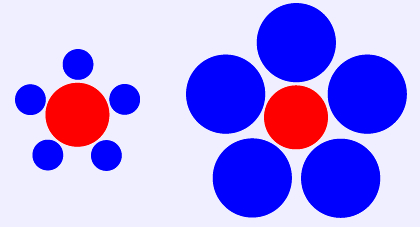
\includegraphics[width=9cm]{Deux_disques_B.jpg}}
\end{minipage}}
%----------------------------------------------

\begin{tikzpicture}[scale=1]

\iffalse
\tkzDefPoint(0,-14.5){A1} \tkzDefShiftPoint[A1](0:18){B1} 
 \tkzDrawPoint  (A1)   \tkzDrawPoint  (B1) 
\tkzDrawSquare[red](A1,B1)
\tkzGetPoints{C1}{D1}
\tkzDefMidPoint(A1,B1)\tkzGetPoint{I}
\tkzDefMidPoint(C1,D1)\tkzGetPoint{J} \draw[red] (I) -- (J) ; 
\tkzDefMidPoint(A1,D1)\tkzGetPoint{K}
\tkzDefMidPoint(B1,C1)\tkzGetPoint{L} \draw[red] (K) -- (L) ; 
\tkzLabelPoints[below](A1)
\tkzLabelPoints[below](B1)
\fi

\node[inner sep=0pt] (sage) at (4.5,-1)
    {\box1 }  ; 
\node[inner sep=0pt] (temps) at (13.5,-1)
      {\box2 }  ; 
\tkzDefPoint(0,0){A} \tkzDefShiftPoint[A](90:-4.55){a} 
% \tkzDrawPoint  (A) 
\tkzDefShiftPoint[A](0:9){m} \tkzDefShiftPoint[m](0:4.5){s} 
\tkzDefPoint(0,2.5){B} \tkzDefShiftPoint[B](90:-4.5){b} 
\tkzDefShiftPoint[B](0:9){n} \tkzDefShiftPoint[n](0:4.5){t} 
\tkzDefPoint(8,3.5){C} \tkzDefShiftPoint[C](90:-4.5){c} 
\tkzDefShiftPoint[C](0:4.5){o} \tkzDefShiftPoint[o](0:4.5){u} 
\tkzDefPoint(9,0){D} \tkzDefShiftPoint[D](90:-4.5){d} 
\tkzDefShiftPoint[d](0:4.5){p} \tkzDefShiftPoint[p](0:4.5){v} 
\tkzDefPoint(8,-1){E}\tkzDefShiftPoint[E](90:-4.5){e} 
\tkzDefShiftPoint[e](0:4.5){q} \tkzDefShiftPoint[q](0:4.5){w} 
\tkzDefPoint(1,-1){F}\tkzDefShiftPoint[F](90:-4.5){f} 
\tkzDefShiftPoint[f](0:9){r}  \tkzDefShiftPoint[r](0:4.5){x} 

\draw [<->](A) -- (B)  arc (180:90:1) -- (C)%
                      arc (90:0:1)   -- (D)
                      arc (0:-90:1)  -- (E) 
            -- (F) arc (-90:-180:1) -- (A) ; 
\draw (a) -- (b) arc (180:90:1) -- (c)        
                      arc (90:0:1)   -- (d)
                      arc (0:-90:1)  -- (e) 
            -- (f) arc (-90:-180:1) -- (a) ; 
\draw (m) -- (n) arc (180:90:1) -- (o)        
                      arc (90:0:1)   -- (p)
                      arc (0:-90:1)  -- (q) 
            -- (r) arc (-90:-180:1) -- (m) ;             
\draw (s) -- (t) arc (180:90:1) -- (u)        
                      arc (90:0:1)   -- (v)
                      arc (0:-90:1)  -- (w) 
            -- (x) arc (-90:-180:1) -- (s) ;  
            
            
               
                  
\iffalse                
%\tkzLabelPoints[left,font=\fontsize{8}{10}\selectfont](m)        
\tkzLabelPoints[left](A) \tkzLabelPoints[left](B) 
\tkzLabelPoints[left](C) \tkzLabelPoints[left](D)   
\tkzLabelPoints[left](E)  
\tkzLabelPoints[left](F)     
\tkzLabelPoints[left](a)     
\tkzLabelPoints[left](b)  
\tkzLabelPoints[left](c) 
\tkzLabelPoints[left](d) 
\tkzLabelPoints[left](e) 
\tkzLabelPoints[left](f) 
\tkzLabelPoints[left](m)     
\tkzLabelPoints[left](n)  
\tkzLabelPoints[left](o) 
\tkzLabelPoints[left](p) 
\tkzLabelPoints[left](q) 
\tkzLabelPoints[left](r) 
\tkzLabelPoints[left](s)     
\tkzLabelPoints[left](t)  
\tkzLabelPoints[left](u) 
\tkzLabelPoints[left](v) 
\tkzLabelPoints[left](w) 
\tkzLabelPoints[left](x) 
\fi

\end{tikzpicture}

\bigskip

\begin{tikzpicture}[scale=1]

\iffalse
\tkzDefPoint(0,-14.5){A1} \tkzDefShiftPoint[A1](0:18){B1} 
 \tkzDrawPoint  (A1)   \tkzDrawPoint  (B1) 
\tkzDrawSquare[red](A1,B1)
\tkzGetPoints{C1}{D1}
\tkzDefMidPoint(A1,B1)\tkzGetPoint{I}
\tkzDefMidPoint(C1,D1)\tkzGetPoint{J} \draw[red] (I) -- (J) ; 
\tkzDefMidPoint(A1,D1)\tkzGetPoint{K}
\tkzDefMidPoint(B1,C1)\tkzGetPoint{L} \draw[red] (K) -- (L) ; 
\tkzLabelPoints[below](A1)
\tkzLabelPoints[below](B1)
\fi

\node[inner sep=0pt] (expliquer) at (4.5,-1)
         {\box3 }  ; 
\node[inner sep=0pt] (dessin) at (13.5,-1)
        {\box4 }  ; 
\tkzDefPoint(0,0){A} \tkzDefShiftPoint[A](90:-4.55){a} 
% \tkzDrawPoint  (A) 
\tkzDefShiftPoint[A](0:9){m} \tkzDefShiftPoint[m](0:4.5){s} 
\tkzDefPoint(0,2.5){B} \tkzDefShiftPoint[B](90:-4.5){b} 
\tkzDefShiftPoint[B](0:9){n} \tkzDefShiftPoint[n](0:4.5){t} 
\tkzDefPoint(8,3.5){C} \tkzDefShiftPoint[C](90:-4.5){c} 
\tkzDefShiftPoint[C](0:4.5){o} \tkzDefShiftPoint[o](0:4.5){u} 
\tkzDefPoint(9,0){D} \tkzDefShiftPoint[D](90:-4.5){d} 
\tkzDefShiftPoint[d](0:4.5){p} \tkzDefShiftPoint[p](0:4.5){v} 
\tkzDefPoint(8,-1){E}\tkzDefShiftPoint[E](90:-4.5){e} 
\tkzDefShiftPoint[e](0:4.5){q} \tkzDefShiftPoint[q](0:4.5){w} 
\tkzDefPoint(1,-1){F}\tkzDefShiftPoint[F](90:-4.5){f} 
\tkzDefShiftPoint[f](0:9){r}  \tkzDefShiftPoint[r](0:4.5){x} 

\draw [<->](A) -- (B)  arc (180:90:1) -- (C)%
                      arc (90:0:1)   -- (D)
                      arc (0:-90:1)  -- (E) 
            -- (F) arc (-90:-180:1) -- (A) ; 
\draw (a) -- (b) arc (180:90:1) -- (c)        
                      arc (90:0:1)   -- (d)
                      arc (0:-90:1)  -- (e) 
            -- (f) arc (-90:-180:1) -- (a) ; 
\draw (m) -- (n) arc (180:90:1) -- (o)        
                      arc (90:0:1)   -- (p)
                      arc (0:-90:1)  -- (q) 
            -- (r) arc (-90:-180:1) -- (m) ;             
\draw (s) -- (t) arc (180:90:1) -- (u)        
                      arc (90:0:1)   -- (v)
                      arc (0:-90:1)  -- (w) 
            -- (x) arc (-90:-180:1) -- (s) ;  
            
            
               
                  
\iffalse                
%\tkzLabelPoints[left,font=\fontsize{8}{10}\selectfont](m)        
\tkzLabelPoints[left](A) \tkzLabelPoints[left](B) 
\tkzLabelPoints[left](C) \tkzLabelPoints[left](D)   
\tkzLabelPoints[left](E)  
\tkzLabelPoints[left](F)     
\tkzLabelPoints[left](a)     
\tkzLabelPoints[left](b)  
\tkzLabelPoints[left](c) 
\tkzLabelPoints[left](d) 
\tkzLabelPoints[left](e) 
\tkzLabelPoints[left](f) 
\tkzLabelPoints[left](m)     
\tkzLabelPoints[left](n)  
\tkzLabelPoints[left](o) 
\tkzLabelPoints[left](p) 
\tkzLabelPoints[left](q) 
\tkzLabelPoints[left](r) 
\tkzLabelPoints[left](s)     
\tkzLabelPoints[left](t)  
\tkzLabelPoints[left](u) 
\tkzLabelPoints[left](v) 
\tkzLabelPoints[left](w) 
\tkzLabelPoints[left](x) 
\fi

\end{tikzpicture}


\ifdefined\COMPLETE
\else
    \end{document}
\fi
